\section{Dipendenze}
Un buon sistema OO dovrebbe basarsi sull'interazione fra gli oggetti e non fra la dipendenza/parentela fra di essi; si vuole avere un’alta coesione ed un basso accoppiamento. Conviene quindi evitare l'uso dell'ereditarietà, che è il tipo più forte di dipendenza, a discapito delle interfacce.
Vogliamo che le classi siano enti più "isolati" possibili e che non dipendano da altri pezzi.
\begin{center}
\textit{Favor composition over inheritance}
\end{center}
L'ereditarietà comporta il fatto che, in caso di cambiamenti radicali ad una classe che sta in alto nella gerarchia, si può rompere tutta la gerarchia perché le figlie devono adattarsi al cambiamento della madre. Se ci sono molte sottoclassi, potrebbe rompersi tutto. Usare le interfacce è buona cosa perché dicono cosa fare ma lasciano libertà di implementazione.Vediamo un esempio:

\begin{lstlisting}
/*classe che elenca una serie di film*/
class ListaFile{
/*classe con metodi di ricerca in una lista*/
	private TrovaFilm f;

	public ListaFilm(){
		f= new CSVMovieFinder("movies.csv");
	}
}
\end{lstlisting}
In questo codice molto semplice sto facendo new CSVMovieFinder, sottoclasse di TrovaFilm, e ho vari problemi. Intanto, se dovesse cambiare l'implementazione del costruttore dovrei aggiornare \textbf{tutti} i costruttori di quella classe, ovunque la abbia dichiarata. Poi, se dovessi pescare i dati no da un CSV ma da un json/SQL dovrei cambiare il tipo di sottoclasse perché la new crea il tipo sbagliato. Se cambiassi TrovaFilm? Insomma, la classe ListaFilm \textbf{dipende} da TrovaFilm tantissimo; un cambiamento a TrovaFilm potrebbe rompere tutto.

Risolvo il problema usando la Dependency Injection.

\subsection{Dependency Injection}
L'idea alla base della Dependency Injection è quella di avere un componente esterno (assembler) che si occupi della creazione degli oggetti e delle loro relative dipendenze e di assemblarle mediante l’utilizzo dell’injection. Questa tecnica mira a minimizzare le dipendeze fra classi.
Questa, può essere realizzata principalmente con tre tecniche che vanno usate in base al contesto:

\subsubsection{Constructor Injection}
La dipendenza viene iniettata tramite l’argomento del costruttore
\begin{lstlisting}
class ListaFilm{
	private TrovaFilm f;

	public ListaFilm(TrovaFilm film){
		f = film; // Constructor injection
	}

	public void qualcosa(){ f. stampaListaAvideo();}
}
\end{lstlisting}
Per risolvere il problema della dipendenza e "staccare" le due classi, posso "iniettare" la dipendenza via costruttore. In altre parole, faccio la new FUORI E NON DENTRO alla classe che necessita di usare l’altra classe. Passo via costruttore una reference ad un oggetto che vive fuori. In questo modo ListaFilm non crea più nulla e non ha più l’ownership dell’oggetto; la classe ListaFilm ha solo una reference che viene gestita altrove; non interessa altro. Notare quindi che in generale, quando è necessario(come in questo caso) che ci sia dipendenza fra classi (ListaFilmdeve usare TrovaFilm) è meglio usare i principi di dependency injection per ridurre l’accoppiamento tra classi.

\subsubsection{Setter Injection}
La dipendenza viene iniettata attraverso un metodo "set".
\begin{lstlisting}
class ListaFilm{
	private TrovaFilm f;

	public void setMovie(TrovaFilm film) {
	f = film;
	}

	public void qualcosa(){ f. stampaListaAvideo();}
}
\end{lstlisting}
Stessi discorsi di prima solo che qui anziché passare al costruttore la dipendenza, la passo via metodo. Nel costruttore creo l'oggetto ma non ho la necessità di usare TrovaFilm, quindi non la passo; piuttosto creo un metodo che mi permette di settare tale variabile. Diciamo quindi che la Constructor Injection mi indica che ho una dipendenza obbligatoria che va usata per forza, la Setter Injection invece mi dice che si ho una dipendenza ma non è cosi "forte", posso anche farne a meno.

\subsubsection{Method Injection}
\begin{lstlisting}
class ListaFilm{
	private TrovaFilm f;

	public void qualcosa(TrovaFilm film) {
		return film.printAll();
	}
}
\end{lstlisting}
Si tratta del tipo più "soft" di injection perché utilizza temporaneamente un'altra dipendenza (classe o interfaccia); la classe non tiene alcuna reference al suo interno di tale dipendenza. Quindi si fa il minimo indispensabile proprio, toccata e fuga via metodo e basta. Il più basso livello.

\subsection{Inversion of control}
Il principio di IoC (detto anche DIP – Dependency Inversion Principle) dice che ogni modulo ad alto o basso livello non deve dipendere da altri moduli ma piuttosto deve dipendere da astrazioni. Si fa inversione di controllo perché si inverte il ruolo di chi gestisce l'applicazione; invece di essere l'app che controlla il flusso di esecuzione, è il framework che controlla il flusso di esecuzione.

\begin{figure}[H]
\centering
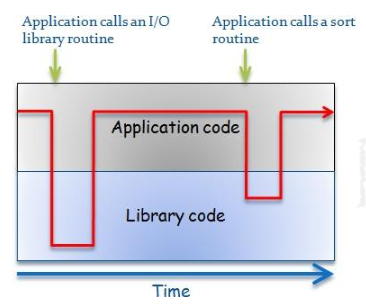
\includegraphics[scale=0.8]{images/ioc1}
\caption{Traditional Program Execution\label{fig:UC3}}
\end{figure}
L’applicazione ha la maggior parte del controllo del flusso di esecuzione (in rosso); questo è un esempio di ciò che normalmente accade. Un'applicazione usa una libreria qualsiasi (libreria numerica, di database...) solo quando ne ha di bisogno ma poi è l'applicazione (scritta dal programmatore) che gestisce. Quindi è il programmatore che tramite il codice dell'applicazione controlla il flusso.

\begin{figure}[H]
\centering
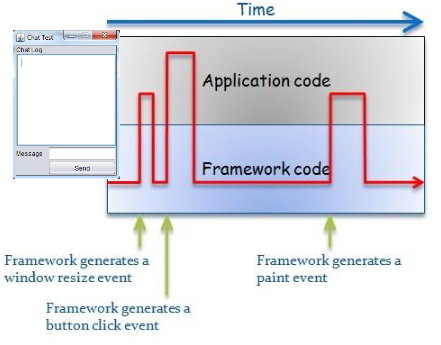
\includegraphics[scale=0.8]{images/ioc2}
\caption{Inversion of Control Execution\label{fig:UC3}}
\end{figure}
In caso di inversione di controllo, c'è un framework che controlla l'intero flusso di una applicazione. Infatti si vede che il flusso appartiene molto alla libreria e poco all'app. Questo accade con le app android ad esempio. Il framework chiama, quando ne ha di bisogno il codice scritto dal programmatore; prima invece era il programmatore chetramite il programma chiamava le funzioni quando voleva lui!

Meglio fare un esempio. Una applicazione Android funziona nell'ambiente Android; quando premo sull'icona di una app c'è il framework (sistema operativo Android) che fa una serie di chiamate a metodi, fa delle new e altre cose per far partire l'app. Il ruolo del programmatore è quello di scrivere una Activity android, cioè il punto di ingresso dell'app (Activity android = il main del C++ per capirci).

Quindi quando l'app parte, il controllo del flusso lo ha in mano il framework (SO Android) perché è lui che chiama i metodi di inizializzazione, gestisce la memoria e gestisce la vita dell'app. Non c'è l'utente che manualmente clicca sull'app, la fa partire invocando i metodi e scegliendo cosa fare.Se ne occupa tutto il sistema operativo.

La dependency injection è una delle tecniche con le quali si può fare inversione di controllo; essa prende il controllo di tutte le azioni base (creazione di oggetti e dipendenze). Famosa è la libreria Spring di java che usa molto questo fatto dell'inizializzazione automatica e cerca di passare il flusso di controllo alla libreria il più possibile.